% Options for packages loaded elsewhere
\PassOptionsToPackage{unicode}{hyperref}
\PassOptionsToPackage{hyphens}{url}
%
\documentclass[
  12pt,
]{article}
\usepackage{lmodern}
\usepackage{amssymb,amsmath}
\usepackage{ifxetex,ifluatex}
\ifnum 0\ifxetex 1\fi\ifluatex 1\fi=0 % if pdftex
  \usepackage[T1]{fontenc}
  \usepackage[utf8]{inputenc}
  \usepackage{textcomp} % provide euro and other symbols
\else % if luatex or xetex
  \usepackage{unicode-math}
  \defaultfontfeatures{Scale=MatchLowercase}
  \defaultfontfeatures[\rmfamily]{Ligatures=TeX,Scale=1}
\fi
% Use upquote if available, for straight quotes in verbatim environments
\IfFileExists{upquote.sty}{\usepackage{upquote}}{}
\IfFileExists{microtype.sty}{% use microtype if available
  \usepackage[]{microtype}
  \UseMicrotypeSet[protrusion]{basicmath} % disable protrusion for tt fonts
}{}
\makeatletter
\@ifundefined{KOMAClassName}{% if non-KOMA class
  \IfFileExists{parskip.sty}{%
    \usepackage{parskip}
  }{% else
    \setlength{\parindent}{0pt}
    \setlength{\parskip}{6pt plus 2pt minus 1pt}}
}{% if KOMA class
  \KOMAoptions{parskip=half}}
\makeatother
\usepackage{xcolor}
\IfFileExists{xurl.sty}{\usepackage{xurl}}{} % add URL line breaks if available
\IfFileExists{bookmark.sty}{\usepackage{bookmark}}{\usepackage{hyperref}}
\hypersetup{
  pdftitle={Plots},
  hidelinks,
  pdfcreator={LaTeX via pandoc}}
\urlstyle{same} % disable monospaced font for URLs
\usepackage[margin=1in]{geometry}
\usepackage{graphicx,grffile}
\makeatletter
\def\maxwidth{\ifdim\Gin@nat@width>\linewidth\linewidth\else\Gin@nat@width\fi}
\def\maxheight{\ifdim\Gin@nat@height>\textheight\textheight\else\Gin@nat@height\fi}
\makeatother
% Scale images if necessary, so that they will not overflow the page
% margins by default, and it is still possible to overwrite the defaults
% using explicit options in \includegraphics[width, height, ...]{}
\setkeys{Gin}{width=\maxwidth,height=\maxheight,keepaspectratio}
% Set default figure placement to htbp
\makeatletter
\def\fps@figure{htbp}
\makeatother
\setlength{\emergencystretch}{3em} % prevent overfull lines
\providecommand{\tightlist}{%
  \setlength{\itemsep}{0pt}\setlength{\parskip}{0pt}}
\setcounter{secnumdepth}{-\maxdimen} % remove section numbering
\usepackage{booktabs}
\usepackage{booktabs}
\usepackage{longtable}
\usepackage{array}
\usepackage{multirow}
\usepackage{wrapfig}
\usepackage{float}
\usepackage{colortbl}
\usepackage{pdflscape}
\usepackage{tabu}
\usepackage{threeparttable}
\usepackage{threeparttablex}
\usepackage[normalem]{ulem}
\usepackage{makecell}
\usepackage{xcolor}

\title{Plots}
\author{}
\date{\vspace{-2.5em}}

\begin{document}
\maketitle

\begin{figure}

{\centering 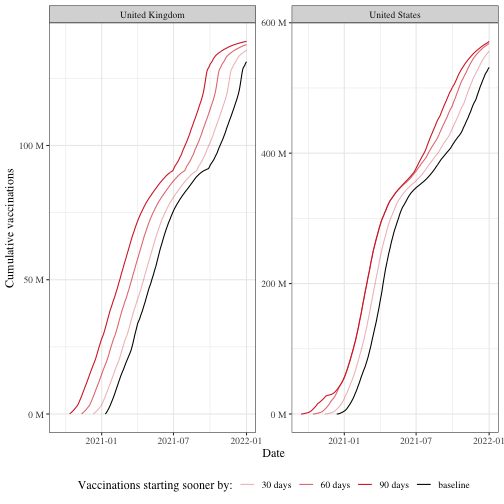
\includegraphics{/Users/Personal/Dropbox/Mac/Documents/HCT Counterfactuals/covid-vaccine-timeline/docs/plots_report_files/figure-latex/cumul-vacc-cfacts-1} 

}

\caption{DJ4 Cumulative vaccine counterfactuals}\label{fig:cumul-vacc-cfacts}
\end{figure}

\begin{table}

\caption{\label{tab:deaths-averted-table}DJ5 Averted deaths}
\centering
\begin{tabular}[t]{lll}
\toprule
Counterfactual scenario & Deaths averted & Deaths averted per 10,000\\
\midrule
\addlinespace[0.3em]
\multicolumn{3}{l}{\textbf{United Kingdom}}\\
\hspace{1em}Vaccines 30 days sooner & -67 [-6,531; 7,941] & -0.01 [-0.97; 1.18]\\
\hspace{1em}Vaccines 60 days sooner & -5,759 [-25,124; 8,630] & -0.86 [-3.75; 1.29]\\
\hspace{1em}Vaccines 90 days sooner & -9,174 [-53,511; 23,387] & -1.37 [-7.98; 3.49]\\
\addlinespace[0.3em]
\multicolumn{3}{l}{\textbf{United States}}\\
\hspace{1em}Vaccines 30 days sooner & 24,962 [12,248; 38,662] & 0.75 [0.37; 1.17]\\
\hspace{1em}Vaccines 60 days sooner & 15,179 [-11,323; 44,089] & 0.46 [-0.34; 1.33]\\
\hspace{1em}Vaccines 90 days sooner & -132 [-30,113; 27,867] & 0.00 [-0.91; 0.84]\\
\bottomrule
\end{tabular}
\end{table}

\begin{figure}

{\centering 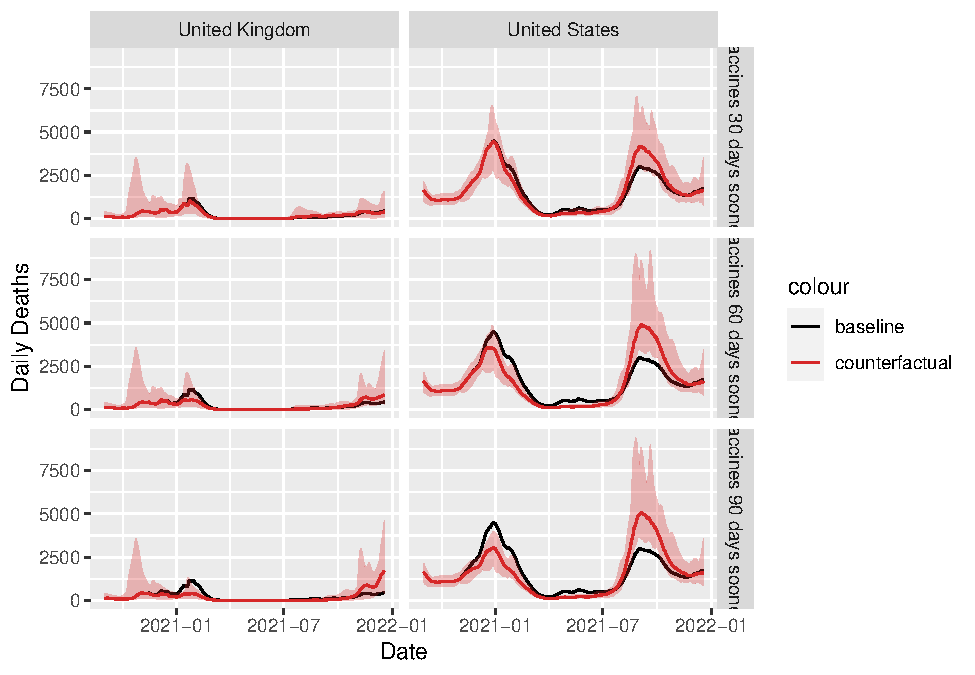
\includegraphics{/Users/Personal/Dropbox/Mac/Documents/HCT Counterfactuals/covid-vaccine-timeline/docs/plots_report_files/figure-latex/deaths-averted-plot-1} 

}

\caption{DJ6 Daily deaths per scenario}\label{fig:deaths-averted-plot}
\end{figure}

\begin{figure}

{\centering 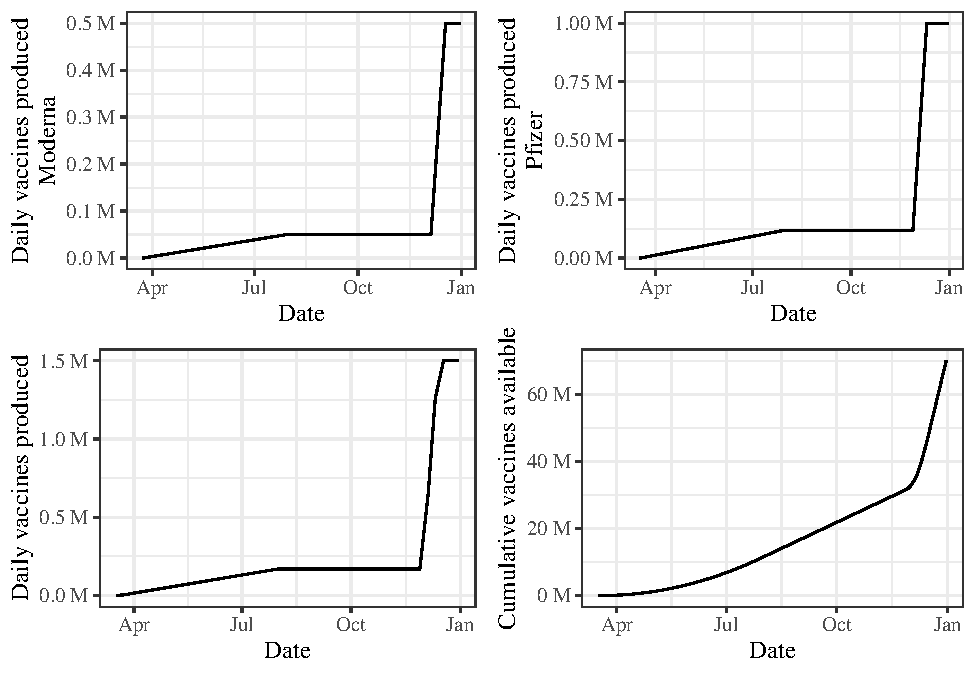
\includegraphics{/Users/Personal/Dropbox/Mac/Documents/HCT Counterfactuals/covid-vaccine-timeline/docs/plots_report_files/figure-latex/prod-assumptions-1} 

}

\caption{DJ9 Vaccine production assumptions}\label{fig:prod-assumptions}
\end{figure}

\begin{figure}

{\centering 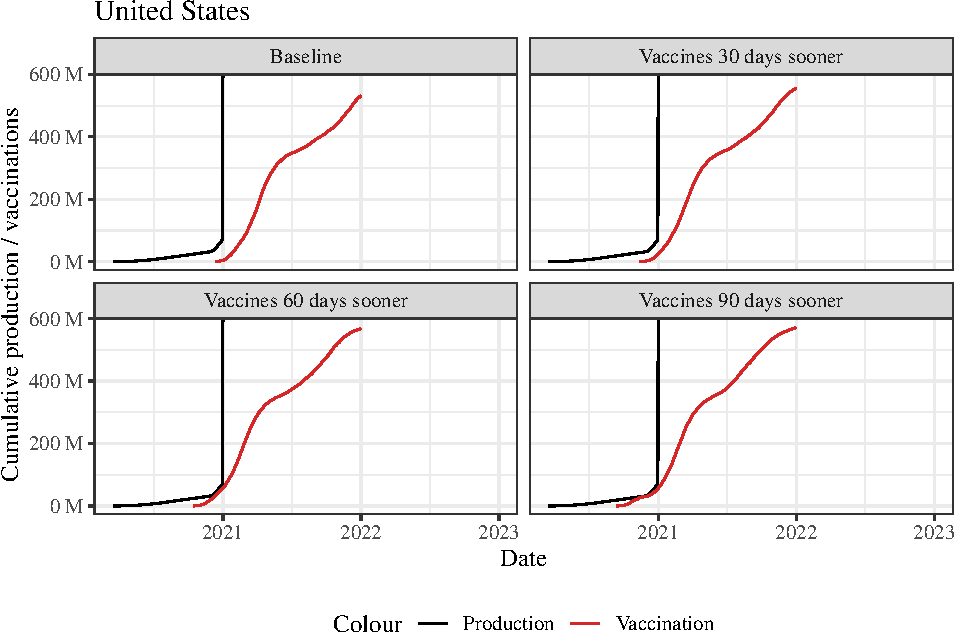
\includegraphics{/Users/Personal/Dropbox/Mac/Documents/HCT Counterfactuals/covid-vaccine-timeline/docs/plots_report_files/figure-latex/prod-cap-1} 

}

\caption{DJ10 Limits from production}\label{fig:prod-cap-1}
\end{figure}
\begin{figure}

{\centering 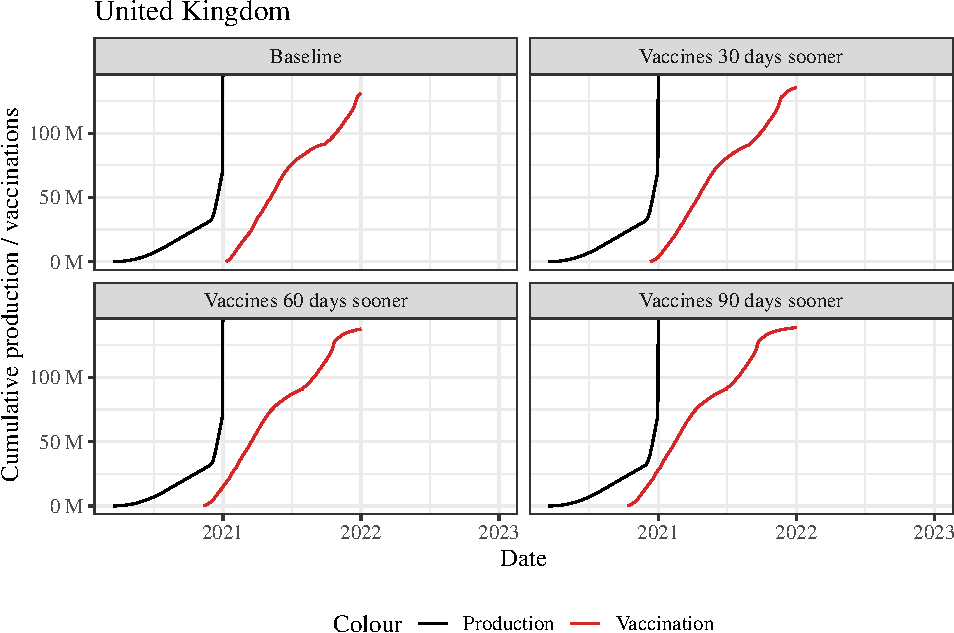
\includegraphics{/Users/Personal/Dropbox/Mac/Documents/HCT Counterfactuals/covid-vaccine-timeline/docs/plots_report_files/figure-latex/prod-cap-2} 

}

\caption{DJ10 Limits from production}\label{fig:prod-cap-2}
\end{figure}

\end{document}
